\section{Viewpoint Analysis}
\label{sec:viewpoint_analysis}

\subsection{Implementation Details}
\label{subsec:implementation-details}

We train a baseline on MOO using an ImageNet-21k~\cite{ridnikImageNet21KPretrainingMasses2021a} pre-trained ViT backbone~\cite{dosovitskiyImageWorth16x162020a} paired with a fully connected classification head.
Following standard ReID practices~\cite{9025455}, images are resized to 256x256 pixels, and augmented with random cropping and horizontal flipping.
The model is trained for 120 epochs using a batch size of 128 (4 images per ID).
We use an SGD optimizer (momentum 0.9, weight decay 1e-4) with a base learning rate of 0.008 and cosine decay, jointly optimizing cross-entropy and triplet losses to constrain the feature space~\cite{9025455}.
We use mean Average Precision (mAP) and Rank-1 accuracy as evaluation metrics, computed using the standard Cumulative Matching Characteristic (CMC) curve.

\subsection{Elevation Impact}
\label{subsec:elevation_impact}

To systematically quantify the impact of viewpoint, we partitioned the dataset into 8 elevation levels ($\theta \in [0^\circ, 85^\circ]$) and 4 azimuthal views (Right, Front, Left, Back) based on our generation grid introduced in section~\ref{subsec:generation-pipeline}.

\subsubsection*{Single-View training}

\Cref{fig:elev1} shows the performance of models trained on a single elevation partition (for query and gallery) and evaluated against all other elevations, in a same-view setup (\ie query and gallery images are drawn from the same partition)

While each model performs best on the partition it was trained on, we observe a distinct asymmetric degradation: models trained at higher elevations generalize significantly better to lower views than vice versa.
Specifically, elevations superior to $30^\circ$ enable robust ReID.
This suggests that, beyond this elevation, top-down views preserve enough shared features across azimuth changes, whereas side views suffer from self-occlusion.

\begin{figure}[tbp]
    \centering
    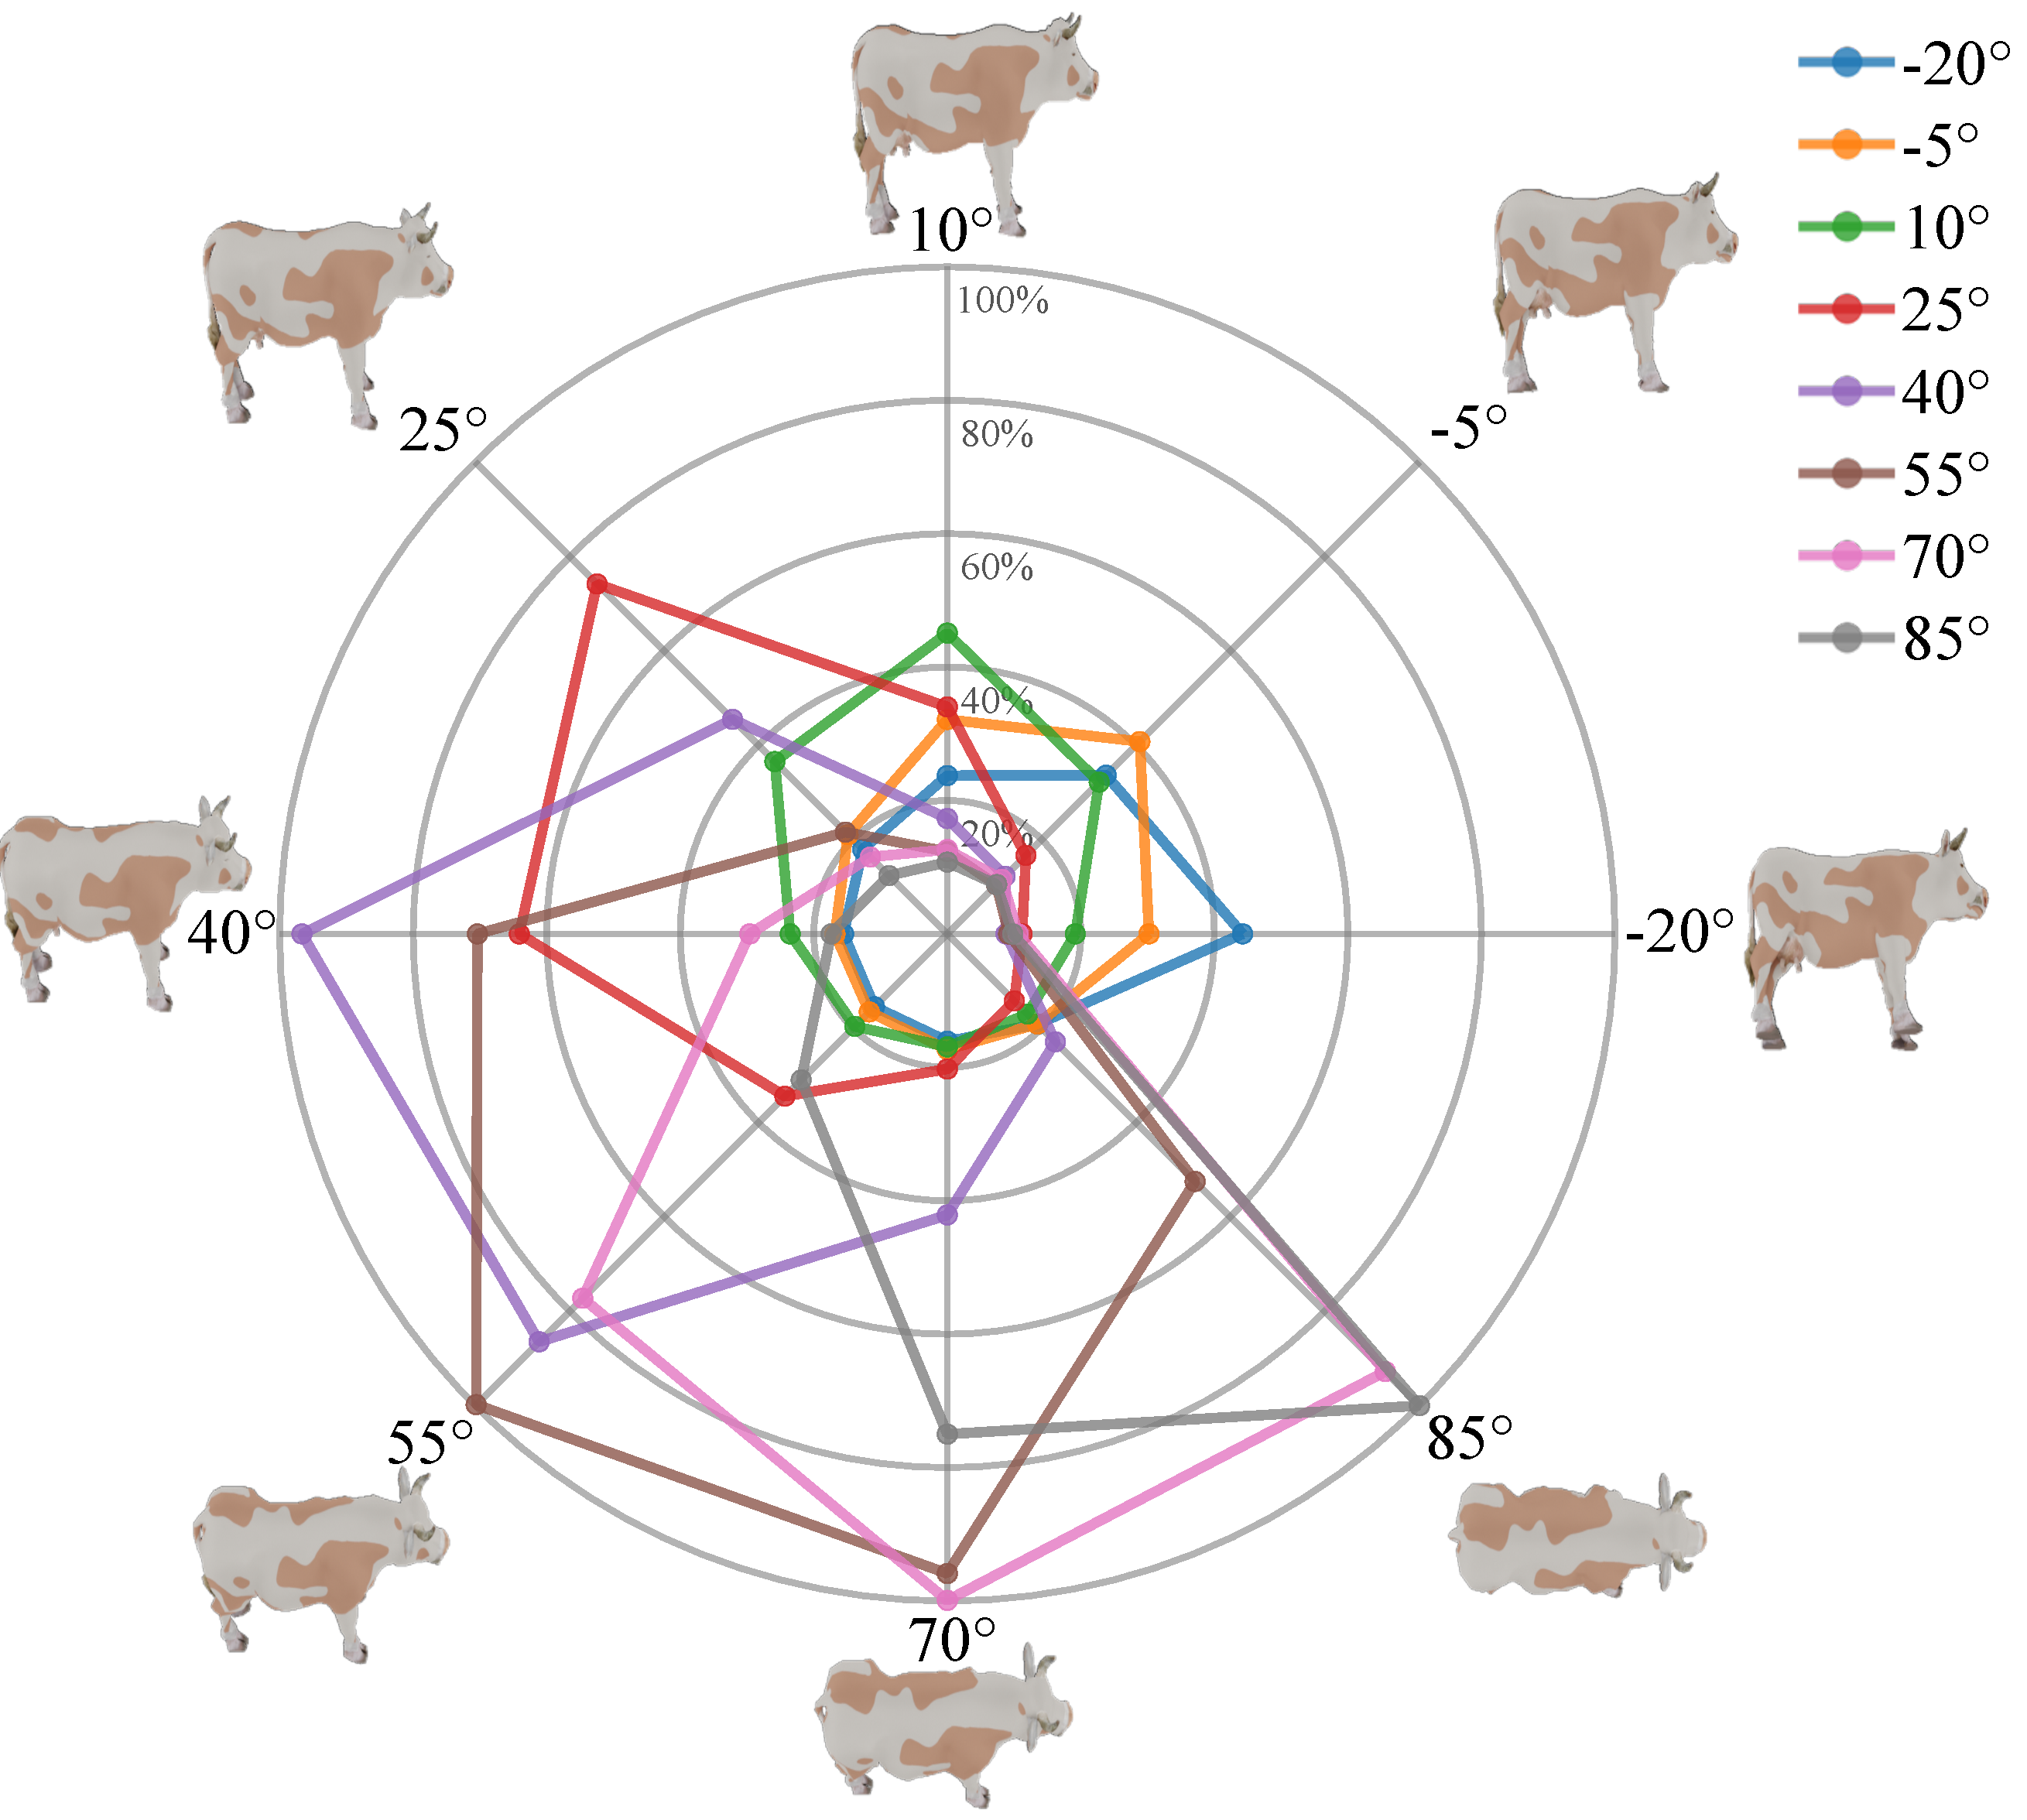
\includegraphics[width=1.0\linewidth]{figure_4}
    \caption{mAP per training elevation range across eight partitions evaluated in a same-view setup, where Query and gallery images share the same elevation.}
    \label{fig:elev1}
\end{figure}

\subsubsection*{All-View training}

We further investigated whether increasing elevation diversity during training improves generalization.
As shown in \Cref{fig:elev2}, training on broader consistently falls short of the theoretical upper bound set by view-specific experts (black dot).
This inability to match specialized models suggests that simply scaling data is insufficient.

\begin{figure}[tbp]
    \centering
    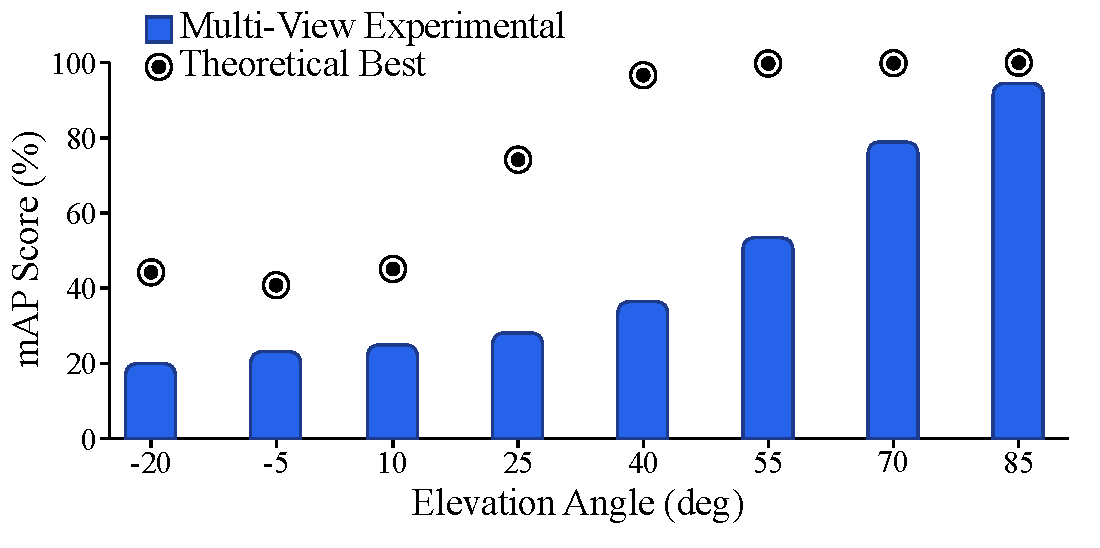
\includegraphics[width=1.0\linewidth]{expert}
    \caption{
        mAP for the best Single-View expert (black dot) and All-View model (blue curve) across eight partitions evaluated in a same-view setup, where Query and gallery images share the same elevation.
    }
    \label{fig:elev2}
\end{figure}

\subsection{Azimuth Impact}
\label{subsec:azimuth-impact}

\Cref{tab:azimuth} demonstrates a clear performance gap where training on lateral views (Right/Left) achieve near-perfect accuracy ($>0.98$), whereas sagittal views (Front/Back) are significantly more challenging.
Naturally, matching the training and inference views yields the best results, but on average, lateral views still outperform sagittal views by $20\%$ mAP and should be prioritized for camera placement when possible.

\begin{table}[t]
    \centering
    \caption{
        mAP across four azimuth training and evaluation scenarios evaluated in a same-view setup, where Query and gallery images share the same view.
    }
    \label{tab:azimuth}

    \scriptsize

    \begin{tabular}{lccccc}
        \toprule
        \diagbox{\textbf{Train}}{\textbf{Test}} & Right         & Left          & Front         & Back          & Average       \\
        \midrule
        Right                                   & \textbf{0.98} & 0.99          & 0.16          & 0.15          & 0.63          \\
        Left                                    & 0.99          & \textbf{0.99} & 0.17          & 0.16          & \textbf{0.65} \\
        Front                                   & 0.42          & 0.42          & \textbf{0.56} & 0.24          & 0.40          \\
        Back                                    & 0.50          & 0.51          & 0.29          & \textbf{0.75} & 0.48          \\
        \bottomrule
    \end{tabular}
\end{table}
